\documentclass[a4paper,11pt,UTF8]{article}
\usepackage{ctex}
\usepackage{amsmath,amsthm,amssymb,amsfonts}
\usepackage{amsmath}
\usepackage[a4paper]{geometry}
\usepackage{graphicx}
\usepackage{microtype}
\usepackage{siunitx}
\usepackage{booktabs}
\usepackage[colorlinks=false, pdfborder={0 0 0}]{hyperref}
\usepackage{cleveref}
\usepackage{esint} 
\usepackage{graphicx}
\usepackage{ragged2e}
\usepackage{pifont}
\usepackage{extarrows}
\usepackage{mathptmx}
\usepackage{float}
\usepackage{caption}
\captionsetup[figure]{name={Figure}}
%opening
\title{模电知识点汇总}
\author{Yuejin Xie \quad U202210333}
\date{}
\begin{document}
\maketitle
\section{Op-Amp}
五种运放模型的汇总:

\begin{figure}[H]
	\begin{minipage}{.69\textwidth}
		\begin{figure}[H] 
			\centering 
			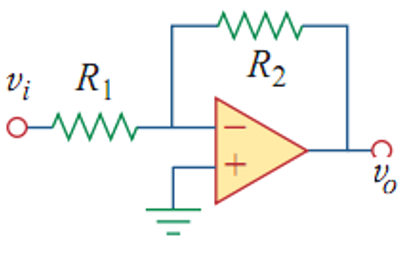
\includegraphics[scale=0.5]{./img/9.1.png}
			\caption{Inverting Amplifier}
		\end{figure}
	\end{minipage}
	\begin{minipage}{.29\textwidth}
		\LARGE{$$
			v_o=-\frac{R_2}{R_1}v_i
			$$}
	\end{minipage}
\end{figure}

\begin{figure}[H]
	\begin{minipage}{.69\textwidth}
		\begin{figure}[H] 
			\centering 
			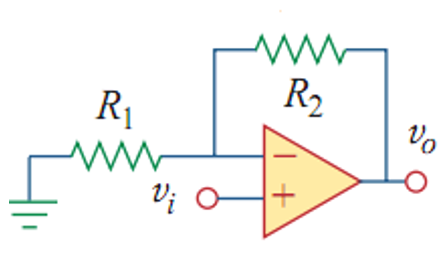
\includegraphics[scale=0.5]{./img/9.2.png}
			\caption{Inverting Amplifier}
		\end{figure}
	\end{minipage}
	\begin{minipage}{.29\textwidth}
		\LARGE{$$
			v_o=(1+\frac{R_2}{R_1})v_i
			$$}
	\end{minipage}
\end{figure}

\begin{figure}[H]
	\begin{minipage}{.69\textwidth}
		\begin{figure}[H] 
			\centering 
			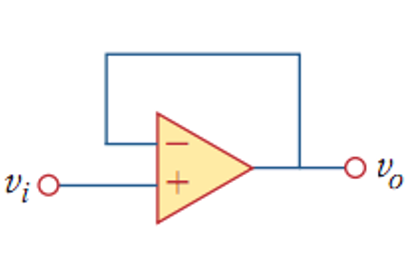
\includegraphics[scale=0.5]{./img/9.3.png}
			\caption{Inverting Amplifier}
		\end{figure}
	\end{minipage}
	\begin{minipage}{.29\textwidth}
		\LARGE{$$
			v_o=v_i
			$$}
	\end{minipage}
\end{figure}

\begin{figure}[H]
	\begin{minipage}{.69\textwidth}
		\begin{figure}[H] 
			\centering 
			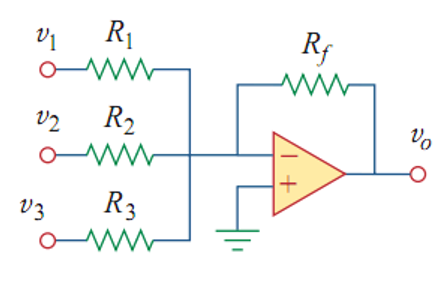
\includegraphics[scale=0.5]{./img/9.4.png}
			\caption{Inverting Amplifier}
		\end{figure}
	\end{minipage}
	\begin{minipage}{.29\textwidth}
		\LARGE{$$
			v_o=-(\frac{R_f}{R_1}v_1+\frac{R_f}{R_2}v_2+\frac{R_f}{R_3}v_3)
			$$}
	\end{minipage}
\end{figure}

\begin{figure}[H]
	\begin{minipage}{.69\textwidth}
		\begin{figure}[H] 
			\centering 
			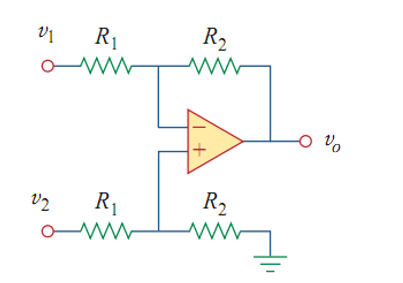
\includegraphics[scale=0.5]{./img/9.5.png}
			\caption{Inverting Amplifier}
		\end{figure}
	\end{minipage}
	\begin{minipage}{.29\textwidth}
		\LARGE{$$
			v_o=\frac{R_2}{R_1}(v_2-v_1)
			$$}
	\end{minipage}
\end{figure}




\end{document}